
\section{Determining the spin effective mass}

Following the method in section~\ref{Sec:Exp:MeasuringSpinMass}, only a couple of portions of the data are suitable for analysis in that they feature more than one identifiable zeros in the oscillations due to the spin term which are suitably strong and well separated from other data. These are a maximal area of the $\alpha$ curve in the $[100]$ direction and a maximal area of the $\beta$ curve in the $[110]$ direction.

We begin by looking at the $\beta$ data by using the cylindrical approximation and then move onto using an expression for $m^*_b$ derived from a polynomial fit to band masses calculated from \ac{DFT}. Figure~\ref{Fig:ResD:DFTBandMassBand4} shows the two fit forms for the band mass used --- an eight order polynomial and the cylindrical approximation --- used as well as in the inset the particular portion of the $\alpha$ band data that was used in the following investigation. As we can see from the inset, we use a relatively small portion of the measured data curve. Detailed in the panels to the right of the figure are the parameters for the two equation forms for the band mass.
%%
\begin{figure}[htbp]
    \begin{center}
        \includegraphics[scale=0.9]{Chapter-dHvABaFe2P2/Figures/Mass/DFTBandMassBand4/DFTBandMassBand4}
        \caption{Band masses calculated from \ac{DFT} of band 4 taken over a range of angles rotating towards the $[100]$ direction. A fit to and order 8 polynomial is shows as well as a comparative fit suing the cylindrical approximation.}
        \label{Fig:ResD:DFTBandMassBand4}
    \end{center}
\end{figure}
%%
Beginning with the cylindrical approximation, figure~\ref{Fig:ResD:Band4SpinMassCylindrical} shows the \ac{FFT} amplitudes for the said portion of the $\alpha$ electron pocket over a range of angles towards the $[100]$ direction as open circles. The shaded areas delimit where we believe the amplitudes go to zero as determined by inspecting the overall shape of the curve and the splitting of the peaks. The upper panel shows the $n=5$ oscillation, with dotted lines showing the bounds using the cylindrical approximation for the band mass. The $n=5$ oscillation most closely matches the zeros in the data with the $n=6$ oscillation which fits reasonably well presented in the middle panel. The lower panel shows the next ($n=7$) and previous oscillations ($n=4$) in order to demonstrate that the $A_S$ curves no longer align well with the data. We note that for negative angles (i.e. where the sample was rotated back beyond $B\parallel[001]$) the amplitude is not symmetric as expected. This has been observed previously for measurement using a similar technique~\cite{Rourke2010b} and the cause has not yet been fully determined. Some possible explanations could be changes in the resistance response of the cantilever as is transitions from flexing upwards to flexing downwards however further investigation will be required to determine this. Taking $g=2$, the spin masses obtained using the cylindrical approximation from the presented curves are $5.01\pm0.05\unitspacing m^*_b$ for $n=5$ and $6.07\pm0.06\unitspacing m^*_b$ for $n=6$.
%%
\begin{figure}[htbp]
    \begin{center}
        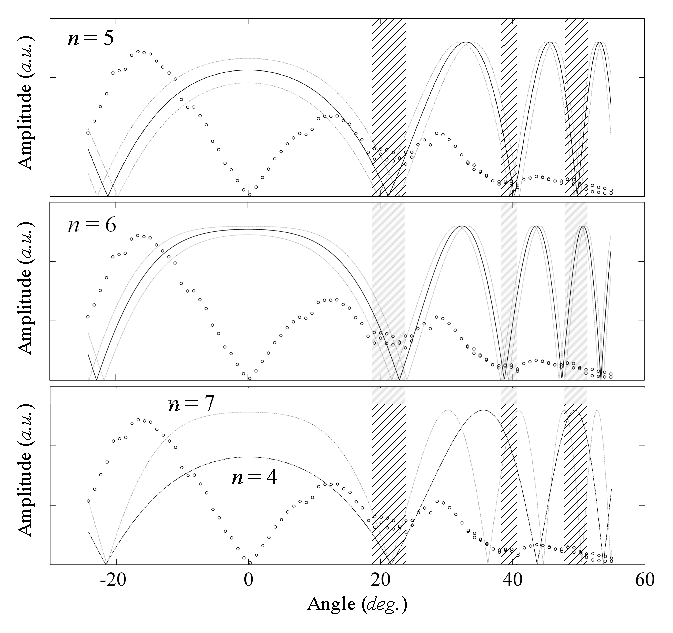
\includegraphics[scale=0.75]{Chapter-dHvABaFe2P2/Figures/Mass/SpinMassBand4Cylindrical/SpinMassBand4Cylindrical}
        \caption{$A_S$ curves calculated for various oscillations using the cylindrical approximation. Open circles are \ac{FFT} amplitudes for $\alpha$ band rotating towards the $[100]$ direction.}
        \label{Fig:ResD:Band4SpinMassCylindrical}
    \end{center}
\end{figure}
%%
We now contrast this with a spin mass determination using a band mass calculated from \ac{DFT}. Figure~\ref{Fig:ResD:SpinMassFromDFTBand4} shows the revised curves with the upper panel showing $n=4$ to be the best fitting with the lower panel demonstrating $n = 3, 5$ do not fit well to the measured data. Now the fit values gives a spin mass of $4.02\pm0.06\unitspacing m^*_b$.
%%
\begin{figure}[htbp]
    \begin{center}
        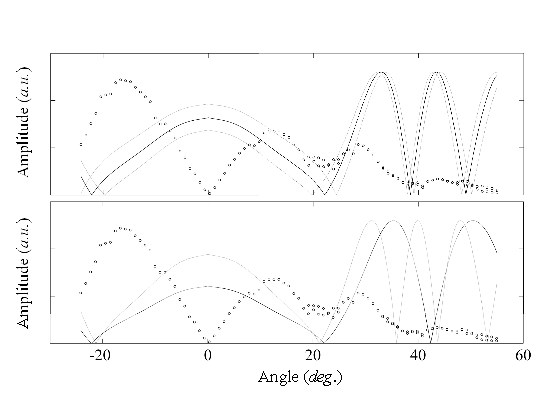
\includegraphics[scale=0.7]{Chapter-dHvABaFe2P2/Figures/Mass/SpinMassBand4/SpinMassBand4}
        \caption{$A_S$ curves calculated for various oscillations using the polynomial fit to \ac{DFT} calculated band masses. Open circles are \ac{FFT} amplitudes for $\alpha$ band rotating towards the $[100]$ direction.}
        \label{Fig:ResD:SpinMassFromDFTBand4}
    \end{center}
\end{figure}
%%
\begin{figure}[htbp]
    \begin{center}
        \includegraphics[scale=0.75]{Chapter-dHvABaFe2P2/Figures/Mass/SpinMassBand3Cylindrical/SpinMassBand3Cylindrical_110}
        \caption{$A_S$ curves calculated for various oscillations using the cylindrical approximation. Open circles are \ac{FFT} amplitudes for $\beta$ band rotating towards the $[110]$ direction.}
        \label{Fig:ResD:SpinMassFromDFTBand3}
    \end{center}
\end{figure}
%%
The second suitable portion of data analysed is that of the maximal extrema of $\beta$ where the field is rotated towards the $[110]$ direction. The \ac{DFT} does not follow exactly the shape of the measured data and leads to a discontinuous jump in the band mass if we strictly follow the maximal orbits --- for this reason we elect to only use the cylindrical approximation since the portion shown appear relatively two-dimensional. Figure~\ref{Fig:ResD:SpinMassCylindricalBand3} shows the reasonable fits for $n=4$ and $n=5$ with the lowest panel showing the oscillations $n=3$ and $n=6$ are clearly not aligned with the measured data. The oscillations $n=4$ and $n=5$ correspond to spin masses of $3.46\pm0.02\unitspacing m^*_b$ and $4.44\pm0.03\unitspacing m^*_b$ respectively.

